\documentclass[11pt]{letter}

\usepackage{graphicx}

\begin{document}

% \maketitle

Tatiana Balbi Fraga \\
Rua Sabiá, 08, Zona Urbana Deslocada,  \\
Chã Grande, CEP:55636-000 \\
tbfraga@proton.me \\

23/04/2024

Juiz de Direito da Vara Única da Comarca de Tamadaré \\
Rua Dr. Leopoldo Lins, S/N, Centro, \\
Tamandaré - PE. CEP:55578-000

Assunto: Contestação à Ação Monitória nº 0001346-98.2022.8.17.3450

Prezado(a) Senhor(a) Juiz(a),

Eu, TATIANA BALBI FRAGA,
brasileira, professora universitária, solteira, inscrita no Cadastro de Pessoas Físicas sob o número 073.815.927-11, e com cédula de identidade de nº 108.229.303 SECC-RJ, venho, por meio deste documento, apresentar minha contestação à Ação Monitória proposta por MONTEBALITO BRASIL EMPRRENDIMENTOS IMOBILIÁRIOS LTDA, atual
denominação da METAMBIENTE BRASIL EMPREENDIMENTOS IMOBILIÁRIOS LTDA, neste documento referido como AUTOR ou METAMBIENTE, nos termos do artigo 702 e seguintes do Código de Processo Civil.

1. DOS FATOS:

1.1 SOBRE O FINANCIAMENTO

Alega o AUTOR que sou devedora da quantia de 113.178,72 reais referente ao contrato CONTRATO DE COMPRA E VENDA DO APARTAMENTO B1-2PS DO CONDOMÍNIO FLAT CLUB MERIDIONAL, datado de 03/02/2011, celebrado entre as partes. Contudo, eu contesto veementemente a existência de qualquer dívida com o AUTOR, devido aos fatos apresentados a seguir.

De acordo com QUADRO RESUMO da PROMESSA DE COMPRA E VENDA celebrada entre as partes e já acostada aos autos, o apartamento que eu comprei estava previsto para ser entregue em 29/12/2014. Conforme e-mail em anexo, em novembro de 2014 eu entrei em contato com o Banco do Brasil e realizei uma avaliação de crédito para já obter o financiamento em dezembro do mesmo ano, momento em que o apartamento deveria estar pronto para entrega. Contudo, a correspondente bancária do Banco do Brasil me informou que para liberar o financiamento, seria necessário um documento do imóvel denominado Habite-se, o qual pode ser obtido unicamente pela empresa junto à prefeitura após o momento em que o imóvel encontra-se pronto para ser habitado.

Eu enviei e-mail para a empresa Metambiente informando que eu estava aguardando o Habite-se para obter o financiamento e solicitei que me informassem quando a empresa estivesse em posse do Habite-se. Ressalto que até então todos os contatos que tive com a empresa, incluindo o recebimento das faturas para pagamento das prestações, eram realizados através de e-mail.

Conforme mostra documento em anexo, eu fui informada sobre a finalização do imóvel apenas em 29/06/2015, quando eu estive na empresa para questionar sobre a disponibilidade do Habite-se, necessário para o financiamento da parcela final e recebimento do imóvel. A empresa me informou que o imóvel já estava pronto desde abril do mesmo ano, mas no entanto, até aquele momento eles não haviam me informado nada por e-mail. Conforme documento em anexo, é possível verificar que o valor cobrado em 29/06/2015 para quitação do pagamento do imóvel através de financiamento do imóvel foi de 188.501,17 reais.

Neste momento procurei novamente o Banco do Brasil para realizar o financimanto, mas este não estava mais aprovando financiamentos de imóveis no Clube Meridional Carneiros, tendo em vista que o condomínio prossui uma área de reserva da marinha. Então, em seguida procurei o Banco Real sob recomendação da pŕopria METAMBIENTE, mas não consegui fazer o financimaneto através deste banco devido às exigencias do mesmo. Então procurei o Banco Bradesco. O Banco Bradesco me entregou documento em anexo com a relação de todos os documentos exigidos para financiamento do imóvel, incluindo documentos meus, documentos do imóvel e documentos da empresa, ou seja do AUTOR. Entreguei ao banco todos os meus documentos solicitados, e solicitei ao AUTOR, na época METAMBIENTE BRASIL EMPREENDIMENTOS IMOBILIÁRIOS LTDA, os documentos do imóvel e os documentos da empresa, conforme recomendação do próprio banco. Como sou funcionária federal e na época não tinha nenhum outro empréstimo ou qualquer limitação de crédito, rapidamente eu tive a aprovação do crédito, contudo para conseguir o financiamento, era necessário entregar ao banco os documentos da empresa e do imóvel.

Conforme mostra imagem abaixo o Habite-se foi averbado pela empresa METAMBIENTE apenas em 28/10/2015

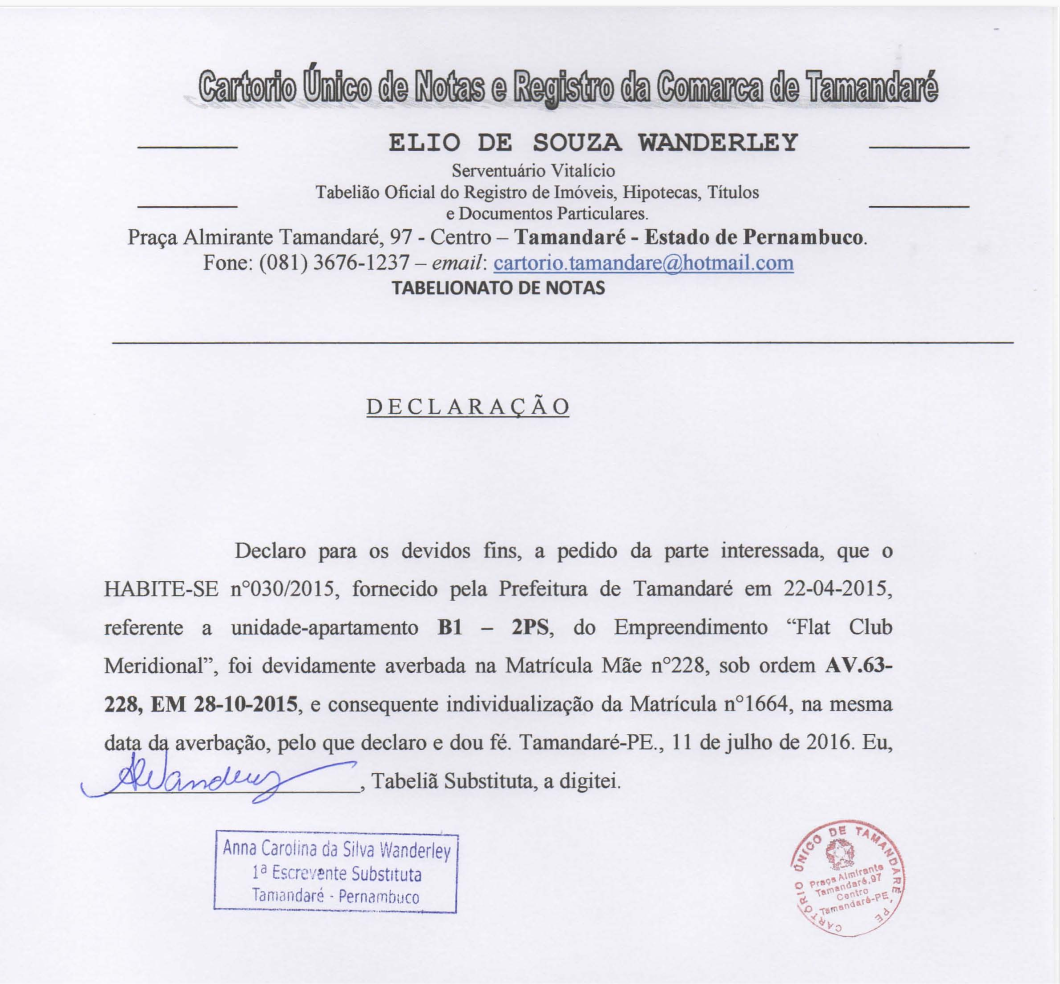
\includegraphics[width=\textwidth]{doc.png}

A averbação do Habite-se era responsabilidade da METAMBIENTE. Até onde eu saiba a averbação do Habite-se é um procedimento necessário para o financiamento do imóvel em qualquer banco. Portanto não seria possível realizar o financimanto antes desta data (28/10/2015).

Quando a METAMBIENTE me entregou todos o último documento solicitado pelo banco, o qual dependia da averbação do Habite-se, eu repassei este documento imediatamente para o Banco Bradesco. O banco então marcou uma visita técnica diretamente com a própria METAMBIENTE para avaliação do imóvel. Depois eu soube que a avaliação do imóvel foi reprovada pelo engenheiro contratado pelo Banco Bradesco para tal finalidade, porque o imóvel não estava identificado. O banco solicitou uma planta do condomínio com a identificação dos imóveis, à METAMBIENTE para poder resolver este problema, mas a empresa não entregou o documento solicitado ao banco. 

Quando eu soube do ocorrido, fiz todo o possível para resolver o problema. Conversei com o gerente responsável e pedi à empresa METAMBIENTE que colocasse uma placa com a devida identificação do imóvel próximo à porta do apartamento a ser financiado, conforme solicitação do gerente responsável. 

Contudo, a empresa METAMBIENTE não atendeu à minha solicitação. Eu acabei perdendo a paciência e fiz uma placa para colocar pessoalmente. Contudo ao falar com a empresa sobre minha atitude planejada, a METAMBIENTE providenciou proximo à porta do apartamento a identificação do imóvel. 

Logo em seguida solicitei nova visita técnica, depois disso o banco solicitou novamente os documentos. Novamente a empresa METAMBIENTE criou dificuldades. Inclusive solicitou que eu pagasse funcionário para adquirir novamente os documentos. Após me entregarem documentação necessária, o financiamento seguiu os trâmites normais e foi finalmente aprovado. O que atrasou o financiamento foram a demora na entrega da documentação por parte da METAMBIENTE assim como a reprovação da primeira visita técnica. 

É necessário verificar que na CLAUSULA III - DA COMPRA E VENDA do Instrumento Particular de Financiamento assinado pela empresa Metambiente Brasil Empreendimentoa Imobiliarios, por mim, Tatiana Balbi Fraga, e pelo Banco Bradesco,  consta no ponto 3.2 que o VENDEDOR DA AO COMPRADOR PLENA, GERAL E IRREVOGÁVEL QUITAÇÃO E TRANSFERE AO COMPRADOR DESDE JÁ A POSSE E DOMINIO DO IMÓVEL ... 

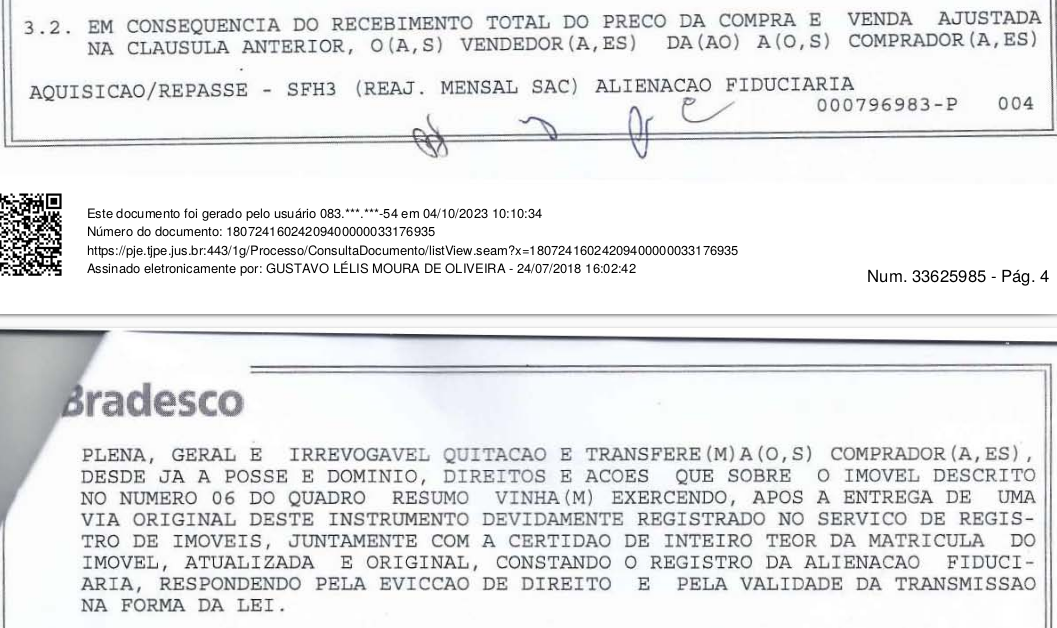
\includegraphics[width=\textwidth]{doc2.png}

Contudo, após o financiamento, a empresa se negou à me entregar as chaves do imóvel, me coagindo à pagar um valor que a empresa alega que eu devia. Devido à cobrança, eu solicitei à empresa METAMBIENTE fatura para pagamento mas a empresa negou me entregar qualquer fatura. Ao invés disso, a empresa METAMBIENTE condicionou a entrega das chaves do imóvel à assinatura de um termo de confissão de dívida. Eu solicitei a fatura com o intuito de procurar um advogado para saber se de fato eu devia algum valor à METAMBIENTE. Caso algum advogado me informasse que o valor era de fato devido eu iria negociar o pagamento com a METAMBIENTE, contudo, assinando um termo de dívida, eu estaria assumindo uma dívida que eu acredito não existir. 

Conforme mostra e-mail, eu tentei ainda solicitar fatura para pagamento do valor de 3.501,17 reais, valor correspondente á diferença entre o valor financiado e o valor cobrado no carta de informação sobre condição do imóvel, contudo a empresa METAMBIENTE se negou a me entregar a fatura. 

Ademais a empresa alegou que, mesmo sem eu receber as chaves do imóvel, eu era responsável pelo pagamento do condomínio e de outras cobranças, tal como o IPTU. Durante um longo período eu paguei todas as taxas e cobranças do imóvel, sem no entanto ter recebido às chaves deste. Os valores pagos por mim são muito superiores à 3.501,17 reais.

Entendendo que de fato havia uma dívida, a empresa METAMBIENTE poderia simplesmente entrar com um processo de cobrança na justiça na época logo após o financimento, mas optou por me coagir, me forçando e entrar com um processo na justiça para solicitação das chaves do imóvel.

De acordo com contrato, eu deveria ter recebido o meu imóvel em 2014, contudo só fui ter acesso ao meu imóvel em 2018, com limiar da justiça. 

1.2 MÁ FE DA PARTE AUTORA

Apesar de ter pleno conhecimento sobre os fatos, o AUTOR tem má fé ao omitir sua responsabilidade por ter provocado atrasos no financiamento, principalmente em função de sua negligência na entrega de documentação necessária para o financiamento. A empresa também tem má fé ao reter as chaves do imóvel para tentar me coagir ao pagamento de valores e multas cobrados pela mesma. Além disso a empresa tem má fé apresentando cobranças absurdas e abusivas, na elaboração da planilha de cobrança, como por exemplo aplicando juro composto e a correção do valor do imóvel pelo INCC entre 27/04/2016 à 04/08/2022, ou seja, mesmo após assinatura do contrato de financiamento em 27/04/2016.

É nítido o fato de que a empresa apresenta diversas cobranças abusivas tentando baseá-las nas cláusulas contratuais. Contudo, nenhum processo pode ser formado no sentido de gerar henriquecimento às custas do REU. De acordo com o artigo 51 da Lei nº 8.078, de 11 de setembro de 1990, são nulas de pleno direito, entre outras, as cláusulas contratuais relativas ao fornecimento de produtos e serviços que: I - impossibilitem, exonerem ou atenuem a responsabilidade do fornecedor por vícios de qualquer natureza dos produtos e serviços ou impliquem renúncia ou disposição de direitos. Nas relações de consumo entre o fornecedor e o consumidor pessoa jurídica, a indenização poderá ser limitada, em situações justificáveis; e IV - estabeleçam obrigações consideradas iníquas, abusivas, que coloquem o consumidor em desvantagem exagerada, ou sejam incompatíveis com a boa-fé ou a eqüidade. 

Portanto, com base no Artigo 702 da Lei nº 13.105 de 16 de Março de 2015, solicito que o juiz condene o AUTOR ao pagamento de multa de dez por cento sobre o valor total da causa.

2. DA RECONVEÇÃO

2.1 DANOS MORAIS E MATERIAIS 
 
Devido à negligência da empresa Montebalito, fui fortemente prejudicada sem poder usufluir do meu imóvel pelo período de 16 meses . Sofri dano material por não poder usufluir ou alugar o imóvel. Portanto solicito reparação por danos materiais referêntes ao pagamento de 16 mensalidades no valor de 1500,00 reais, somando 24.000,00 reais corrigidos de acordo com atualização monetária. Também sofri danos morais já que fiquei enormermente constrangida com a coação e com toda esta situação além de muito estressada e desiludida com a compra do meu imóvel. Toda esta questão desnecessártia gerada pela empresa Metambiente transfomou a alegria de adquirir um patrimônio com tanto esforço em problemas e constragimentos. Portanto solicito indenização a ser definida por este juizo não inferior a 20.000,00 reais. 

2.2 COBRANÇA INDEVIDA - PAGAMENTO EM DOBRO

Além dos motivos alencados anteriormente que comprovam que eu não fui responsável pelo atraso no pagamento da parcela final, o contrato de financiamento e quitação do imóvel foi firmado em 27/04/2016. De acordo com a Artigo 206 da Lei nº 10.406 de 10 de Janeiro de 2002, caso houvesse alguma dívida pendente, está estaria prescrita após um período de 5 anos, ou seja em 2021.

Com base no artigo 940 da Lei no 10.406, de 10 de janeiro de 2002, peço pagamento do valor em dobro ao valor total cobrado pela empresa Montebalito, totalizando 226.357,44.

Caso o juiz entenda que existe algum valor a ser pago que seja inferior ao valor cobrado pelo AUTOR, peço pagamento em dobro relativo à diferença entre o valor cobrado e o valor definido como devido. 

3. DOS PEDIDOS

Diante do exposto, requer-se:
3.1. O acolhimento da presente contestação, para que seja extinto o processo monitório sem resolução de mérito, nos termos do artigo 485, VI, do Código de Processo Civil.

3.2.A condenação do AUTOR ao pagamento de:

	44.000,00 reais correspondente aos danos morais e materiais;
	226.357,44 relativos ao pagamento em dobro do valor da cobrança indevida;
	multa de 10\% do valor da causa devido à má fé da parte autora.
	
3.3. Citação do Banco Bradesco identificado no Instrumento Particular de Financiamento anexado a este processo para que este apresente explicações sobre todo o processo de financiamento, incluindo a não existência de qualquer impedimento relacionado a minha documentação para aprovação do crédito, a reprovação da primeira visita técnica, e a demora na entrega dos documentos solicitados pelo banco, relativos ao imóvel e à empresa. 

	
Junto a esta, apresento documentos que comprovam a improcedência dos fatos alegados pelo autor.

Nestes termos, \\
Dra. Tatiana Balbi Fraga \\
Professora Universitária

\begin{center}
             \_\_\_\_\_\_\_\_\_\_\_\_\_\_\_\_\_\_\_\_\_\_\_\_\_\_\_\_\_\_\_\_\_\_\_\_\_\_\_\_\_\_\_\_\_\_\_\_\_\_\_\_\_\_\_\_\_\_\_\_\_\_\_\_\_\_\_\_\_\_
    
\end{center}  
          
Att.,

Tatiana Balbi Fraga

\end{document}

